\chapter{Degree, Linking Numbers and Index of Vector Fields}
Let $f:N^n\to M^n$ be a smooth map between compact connected oriented manifolds 
of the same dimension $n$. We have the commutative diagram
\begin{equation}\label{eq:11-1}
  \begin{tikzcd}
    H^n(M) \arrow[d, "\simee"']\rar{H^n(f)} & H^n(N)\arrow[d, "\simee"']\\
    \RR \rar{\R{deg}(f)} & \RR 
  \end{tikzcd}
\end{equation}

where the vertical isomorphisms are given by integration over $M$ and $N$ respectively; cf. 
Corollary \ref{corollary:10-14}. The lower horizontal arrow is multiplication by the
real number $\R{deg}(f)$ that makes the diagram commutative. Thus for $\omega\in\Omega^n(M)$,
\begin{align}\label{eq:11-2}
  \int_N f^*\omega = \R{deg}(f)\int_M \omega.
\end{align}

This formulation can be generalized to the case where $N$ is not connected:

\begin{proposition}\label{prop:11-1}
  Let $f:N^n\to M^n$ be a smooth map between compact $n$-dimensional oriented manifolds 
  with $M$ connected. There exists a unique $\R{deg}(f)\in\RR$ such that \eqref{eq:11-2} holds 
  for all $\omega\in\Omega^n(M)$. We call $\R{deg}(f)$ the degree of $f$.
\end{proposition}

\begin{proof}
  We write $N$ as a disjoint union of its connected components $N_1, \cdots, N_k$ and
and denote the restriction of $f$ to $N_j$ by $f_j$. We have already defined $\R{deg}(f_i)$;
we set
\begin{align}\label{eq:11-3}
  \R{deg}(f) = \sum_{j=1}^{k }{\R{deg}(f_j)}.
\end{align}

Thus for $\omega\in\Omega^n(M)$, we have, 
\begin{align*}
  \int_N f^*\omega 
  = \sum_{j=1}^{k}{\int_{N_j}f_j^*\omega} 
  = \sum_{j=1}^{k}{\R{deg}(f_j)\int_M\omega} 
  = \R{deg}(f)\int_M\omega.
\end{align*}
\end{proof}

\begin{corollary}\label{corollary:11-2}
  $\R{deg}(f)$ depends only on the homotopy class of $f:N\to M$.
\end{corollary}

\begin{proof}
  By \eqref{eq:11-3} we can restrict ourselves to the case where $N$ is connected.
The assertion then follows from diagram (1), since $H^n(f)$ depends only on the
homotopy class of $f$.
\end{proof}

\begin{corollary}\label{corollary:11-3}
  Suppose $N^n\xra[f]M^n\xra[g]P^n$ are smooth maps between $n$-dimensional compact 
  oriented manifolds and that $M$ and $P$ are connected. Then 
  \begin{align*}
    \R{deg}(gf) = \R{deg}(g)\R{deg}(f).
  \end{align*}
\end{corollary}

\begin{proof}
  For $\omega\in\Omega^n(P)$, 
  \begin{align*}
    \R{deg}(gf)\int_p\omega 
    & = \int_N(gf)^*(\omega)
      = \int_N f^*(g^*(\omega)) \\
    & = \R{deg}(f)\int_M g^*(\omega)
      = \R{deg}(f)\R{deg}(g)\int_P\omega.
  \end{align*}
\end{proof}

\begin{remark}\label{remark:11-4}
  If $f:M^n\to N^n$ is a smooth map of a connected compact orientable
manifold to itself then $\R{deg}(f)$ can be defined by chosing an orientation of $M$ and
using it at both the domain and range. Change of orientation leaves $\R{deg}(f)$.
unaffected.
\end{remark}

We will show that $\R{deg}(f)$ takes only integer values. This follows from an important geometric 
interpretation of $\R{deg}(f)$ which uses the concept of regular value. In general $p\in M$ is said 
to be a \Index{regular value} for the smooth map $f:N^n\to M^n$ if
\begin{align*}
  D_qf:T_pN\to T_pM
\end{align*}

is surjective for all $q\in f^{-1}(p)$. In particular, points in the complement of $f(N^n)$
are regular values. Regular values are in rich supply:

\begin{theorem}[Brown-Sard]\label{theorem:11-5}\index{Brown-Sard theorem}\index{Sard theorem}
  For every smooth map $f: N^n \to M^m$ the set of regular values is dense in $M^m$.
\end{theorem}

When proving Theorem \ref{theorem:11-5} one may replace $M^m$ by an open subset $W\sseq M$
diffeomorphic to $\RR^n$, and replace $N^n$ by $f^{-1}(W)$. This reduces Theorem \ref{theorem:11-5}
to the special case where $M^m = \RR^m$.

In this case one shows, that almost all points in $\RR^m$ (in the Lebesgue sense) are
regular values. By covering $N^n$ with countably many coordinate patches and
using the fact that the union of countably many Lebesgue null-sets is again a
null-set, Theorem \ref{theorem:11-5} therefore reduces to the following result:

\begin{theorem}[Sard, 1942]\label{theorem:11-6}
  Let $f:U\to\RR^m$ be a smooth map defined on an open set $U\sseq\RR^n$ and let
  \begin{align*}
    S = \{x\in U\big| \text{rank} D_xf < m\}.
  \end{align*}

  Then $f(S)$ is a Lebesgue null-set in $\RR^m$.
\end{theorem}

Note that $x\in U$ belongs to $S$ if and only if every $m\times m$ submatrix of the Jacobi
matrix of $f$, evaluated at $x$, has determinant zero. Therefore $S$ is closed in $U$ and
we can write $S$ as a union of at most countably many compact subsets $K\sseq S$.
Theorem \ref{theorem:11-6} thus follows if $f(K)$ is a Lebesgue null-set for every compact
subset $K$ of $S$. We shall only use and prove these theorems in the case $m = n$,
where they follow from

\begin{proposition}\label{prop:11-7}
  Let $f:U\to \RR^n$ be a $C^1$-map defined on an open set $U\sseq \RR^n$,
and let $K\sseq S$ be a compact set such that $\det(D_xf) = 0$ for all $x\in K$. Then
$f(K)$ is a Lebesgue null-set in $\RR^n$.
\end{proposition}

\begin{proof}
  Choose a compact set $L\sseq U$ which contains $K$ in the interior, $K\sseq L$. Let 
  $C>0$ be a constant such that 
  \begin{align}\label{eq:11-4}
    \sup_{\xi\in L}\|\grad_\xi f_j\| \leq C\qquad (1\le j \le n).
  \end{align}

  Here $f_j$ is the $i$-th coordinate function of $f$, and $\|\cdot\|$ denotes the Euclidean norm.
  Let 
  \begin{align*}
    T = \prod_{i=1}^n [t_i, t_i + a]
  \end{align*}

  be a cube such that $K\sseq S$, and let $\epsilon>0$. Since the functions $\partial f_j/\partial x_i$ 
  are uniformly continuous on $L$, there exists a $\delta >0$ such that
  \begin{align}\label{eq:11-5}
    \|x-y\|\le \delta \implies 
    \left|\frac{\partial f_j }{\partial x_i }(x) - \frac{\partial f_j }{\partial x_i}(y)\right|\le \epsilon,
    (1\le i,j\le n \text{ and } x, y\in L).
  \end{align}
  We subdivide $T$ into a union of $N^n$ closed small cubes $T_l$ with side length $\frac aN$,
  and choose $N$ so that
  \begin{align}\label{eq:11-6}
    \R{diam}(T_1) = \frac{a\sqrt{n}}{N}\le \delta, \qquad T_1\cap K \neq 0\implies T_1\sseq L.
  \end{align}
  For a small cube $T_l$ with $T_1\cap K\neq \ns$ we pick $x\in T_l\cap K$. If $y\in T_l$ the 
  mean value theorem yields points $\xi_j$ on the line segment between $x$ and $y$ for which
  \begin{align}\label{eq:11-7}
    f_j(y) - f_j(x) 
    = \sum_{i=1}^{n }{\frac{\partial f_j }{\partial x_i }(\xi_j)(y_i - x_i)}.
  \end{align}

  Since $\xi_j\in T_l\sseq L$, the Cauchy-Schwarz inequality and \eqref{eq:11-4} give
  \begin{align*}
    |f_j(y) - f_j(x)| \le C\|y-x\|
  \end{align*}
  and by \eqref{eq:11-6}, 
  \begin{align}\label{eq:11-8}
    \|f(y) - f(x)\| \le C\|y-x\| \le C\sqrt{n}\R{diam}(T_1) = \frac{anC}{N}.
  \end{align}
  Formula \eqref{eq:11-7} can be rewritten as
  \begin{align}\label{eq:11-9}
    f(y) = f(x) + D_x f(y-x) + z,
  \end{align}
  where $z = (z_1, \cdots, z_n)$ is given by 
  \begin{align*}
    z_j = \sum_{i=1}^{n }{\left(\frac{\partial f_j }{\partial x_i }(\xi_j) - \frac{\partial f_j }{\partial x_i }(x_i)\right) (y_i - x_i)}.
  \end{align*}
  By \eqref{eq:11-6}, $\|\xi_j-x\|\le \delta$, so that $|z_j|\le \epsilon n\frac aN$. Hence 
  \begin{align}\label{eq:11-10}
    \|z\| \le \epsilon \frac{an\sqrt{n}}{N}.
  \end{align}
  Since the image of $D_xf$ is a proper subspace of $\RR^n$, we may choose an affine
  hyperplane $H\sseq \RR^n$ with
  \begin{align*}
    f(x) + \im (D_xf)\sseq H.
  \end{align*}
  By \eqref{eq:11-9} and \eqref{eq:11-10} the distance from $f(y)$ to $H$ is less than $\epsilon \frac{an\sqrt{n}}{N}$. 
  Then \eqref{eq:11-8} implies that $f(T_l)$ is contained in the set $D_l$ consisting of all points $q\in\RR^n$ whose
  orthogonal projection $\R{pr}(q)$ on $H$ lies in the closed ball in $H$ with radius $\epsilon \frac{anC}{N}$
  and centre $f(x)$ and $\|q-\R{pr}(q)\|\le \epsilon \frac{an\sqrt{n}}{N}$. For the Lebesgue measure $\mu_n$ on $\RR^n$
  we have
  \begin{align*}
    \mu_n(D_i) 
      = 2\epsilon \frac{an\sqrt{n}}{N} \left(\frac{anC }{N }\right)^{n-1}
        \mkern-15mu\R{vol}(D^{n-1})
      = \epsilon \frac{c}{N^n}
  \end{align*}
  where $c = 2a^nn^{n+\frac12}C^{n-1}\R{Vol}(D^{n-1})$. For evry small cube $T_l$ with $T_l\cap K\neq\ns$
  we now have $\mu_n(f(T_l))\le \epsilon\frac{c}{N^n}$. Since there are at most $N^n$ such small cubes $T_l$,
  $\mu_n(f(K))\le c\epsilon$. This holds for every $\epsilon>0$ and proves the assertion.
\end{proof}

\begin{lemma}\label{lemma:11-8}
  Let $p\in M^n$ be a regular value for the smooth map $f:N^n\to M^n$, with $N^n$ compact. 
  Then $f^{-1}(p)$ consists offinitely many points $q_1, \cdots, q_k$. Moreover, there exist 
  disjoint open neighborhoods $V_i$ of $q_i$ in $N^n$, and an open neighborhood $U$ of $p$ in $M^n$,
  such that
  \begin{enumerate}[(i)]
    \item $f^{-1}(U) = \cup_{i=1}^k V_i$.
    \item $f_i$ maps $V_i$ diffeomorphically onto $U$ for $1\le i\le k$.
  \end{enumerate}
\end{lemma}

\begin{proof}
  For each $q\in F^{-1}(U)$, $D_qf:T_qN\to T_q M$ is an isomorphism. From the
inverse function theorem we know that $f$ is a local diffeomorphism around $q$. In
particular $q$ is an isolated point in $f^{-1}(p)$. Compactness of $N$ implies that $f^{-1}(p)$
consists of finitely many points $q_1, \cdots, q_k$. We can choose mutually disjoint open
neighborhoods $W_i$ of $q_i$ in $N$, such that $f$ maps $W_i$ diffeomorphically onto an
open neighborhood $f(W_i)$ of $p$ in $M$. Let
\begin{align*}
  U = \left(\bigcap_{i=1}^k f(W_i)\right)
    - f\left(N - \bigcup_{i=1}^k W_i\right) 
\end{align*}
Since $N - \bigcup_{i=1}^k W_i$ is closed in $N$ and therefore compact $f(N - \bigcup_{i=1}^k W_i)$ is 
also compact. Hence $U$ is an open neighborhood of $p$ in $M$. We then set 
$V_i = W_i\cap f^{-1}(U)$.
\end{proof}

Consider a smooth map $f:N^n\to M^n$ between compact $n$-dimensional oriented
manifolds, with $M$ connected. For a regular value $p\in M$ and $q\in f^{-1}(p)$, define
the local index
\begin{align}
  \R{Ind}(f, g) = \left\{\begin{aligned}
    & 1   && \text{ if } D_qf:T_pN \to T_pM \text{ preserves orientation } \\
    & -1  && \text{ otherwise. }
  \end{aligned}\right.
\end{align}

\begin{theorem}\label{theorem:11-9}
  In the situation above, and for every regular value $p$, 
  \begin{align*}
    \R{deg}(f) = \sum_{q\in f^{-1}(p)}{\R{Ind}(f; q)}.
  \end{align*}
  In particular $\R{deg}(f)$ is an integer. 
\end{theorem}

\begin{proof}
  Let $q_i, V_i$, and $U$ be as in Lemma \ref{lemma:11-8}. We may assume that $U$ and
hence $V_i$ connected. The diffeomorphism $f_{|V_i}:V_i\to U$ is positively or negatively
oriented, depending on whether $\R{Ind}(f; q)$ is 1 or -1. Let $\omega\in\Omega^n(M)$ be an
$n$-form with
\begin{align*}
  \supp_M(\omega)\sseq U, \qquad \int_M \omega = 1.
\end{align*}

Then $\supp_N(f^*(\omega))\sseq f^{-1}(U) = V_1\cup\cdots\cup V_k$, and we can write 
\begin{align*}
  f^*(\omega) = \sum_{i=1}^k{\omega_i}
\end{align*}
where $\omega_i\in\Omega^n(N)$ and $\supp(\omega_1)\sseq U$. Here $\omega_{i|V_i} = (f_{|V_i})^*(\omega_{|U})$. The 
formula is a consequence of the following calculation:
\begin{align*}
  \R{deg}(f) 
  & = \R{deg}(f)\int_M\omega 
    = \int_Mf^*(\omega) 
    = \sum_{i=1 }^{k }{\int_N \omega_i}
    = \sum_{i=1}^{k}{\int_{V_i} (f_{|V_i})^*(\omega_{|U})} \\
  & = \sum_{i=1 }^{k }{\R{Ind}(f; q_i)\int_U \omega_{|U} }
    = \sum_{i=1}^{k}{\R{Ind}(f; q_i)}.
\end{align*} 

In the special case where $f^{-l}(p) = 0$ the theorem shows that $\R{deg}(f) = 0$ (in the
proof above we get $f^*(\omega) = 0$). Thus we have 
\end{proof}

\begin{corollary}\label{corollary:11-10}
  If $\R{deg}(f)\neq 0$, then $f$ is surjective.
\end{corollary}

\begin{proposition}\label{prop:11-11}
  Let $F:P^{n+1}\to M^n$ be a smooth map between oriented smooth
  manifolds, with $M^n$ compact and connected. Let $X\sseq P$ be a compact domain with
  smooth boundary $N^n =\partial x$, and suppose $N$ is the disjoint union ofsubmanifolds
  $N_i^n,\cdots, N_k^n$. If $f_i = F_{|N_i}$, then
  \begin{align*}
    \sum_{i=1 }^{k }{\R{deg}(f_i)} = 0.
  \end{align*}
\end{proposition}

\begin{proof}
  Let $f = F_{|N}$ so that 
  \begin{align*}
    \R{deg}(f) = \sum_{i=1}^{k}{\R{deg}(f_i)}.
  \end{align*}
  On the other hand, if $\omega\in\Omega^n(M)$ has $\int_M \omega=1$, then 
  \begin{align*}
    \R{deg}(f) = \int_N f^*(\omega)
    = \int_X \dd F^*(\omega)
    = \int_X F^*(\dd\omega)
    = 0
  \end{align*}
  where the second equation is from Theorem \ref{theorem:10-8}.
\end{proof}

We shall give two applications of degree. We first consider linking numbers, and
then treat indices of vector fields.

\begin{definition}\label{def:11-12}\index{linking number}
  Let $J^d$ and $K^l$ be two disjoint compact oriented connected smooth submanifolds of $\RR^{n +1}$, 
  whose dimensions $d\ge 1, l\ge 1$ satisfy $d + l = n$. Their linking number is the integer
  \begin{align*}
    \R{lk}(J, K) = \R{deg}(\Psi_{J, K})
  \end{align*}
  where 
  \begin{align*}
    \Psi = \Psi_{J, K}:J\times K\to S^{n};\qquad \Psi(x, y) = \frac{y-x}{\|y-x\|}.
  \end{align*}
\end{definition}

Here $J\times K$ is equipped with the product orientation (cf. Remark \ref{remark:9-20}) and $S^n$ 
is oriented as the boundary of $D^{n+1}$ with the standard orientation of $\RR^{n+1}$. We note
that $\R{lk}(J, K)$ changes sign when the orientation of either $J$ or $K$ is reversed.

\begin{proposition}\label{prop:11-13}\;\par 
  \begin{enumerate}[(i)]
    \item $\R{lk}(K^l, J^d) = (-1)^{(d+1)(l+1)}\R{lk}(J^d, K^l)$.
    \item If $J$ and $K$ can be separated by a hyperplane $H\subset\RR^{n+1}$ then $\R{lk}(J, K) = 0$.
    \item Let $g_t$ and $h_t$ be homotopies of the inclusions $g_0:J\to\RR^{n+1}$ and $h_0:K\to\RR^{n+1}$
      to smooth embeddings $g_1$ and $h_1$, such that $g_t(J)\cap h_t(K) = \ns$ for all $t\in[0, 1]$. Then 
      $\R{lk}(J, K) = \R{lk}(g_1(J), h_1(K))$.
    \item Let $\Phi:P^{n+1}\to\RR^{n+1}-J$ be a smooth map with $P$ oriented. Given a compact domain 
      $R\sseq P$ with smooth boundary $\partial R$, let $Q_1, \cdots, Q_k$ be the connected components 
      of $\partial R$. Suppose each $\Phi_{|Q_j}$ is a smooth embedding. If $K_i = \Phi(Q_i)$, then 
      \begin{align*}
        \sum_{i=1 }^{k }{\R{lk}(J; K_i)} = 0.
      \end{align*}
  \end{enumerate}
\end{proposition}

\begin{proof}
  We look at the commutative diagram 
  \begin{center}
    \begin{tikzcd}
      J\times K \rar{\Psi_{J, K}}\dar{T} & S^n \dar{A}\\
      K\times J \rar{\Psi_{K, J}} & S^n
    \end{tikzcd}
  \end{center}

  where $T$ interchanges factors and $A$ is the antipodal map $Av = -v$. Then (i)
  follows from Corollary \ref{corollary:11-3} upon using that
  \begin{align*}
    \R{deg}(T) = (-1)^{dl}, \qquad \R{deg}(A) = (-1)^{n+1} = (-1)^{d+l+1}.
  \end{align*}

  In the situation of (ii) the image of $\Psi$ will not contain vectors parallel to $H$, and
  the assertion follows from Corollary \ref{corollary:11-10}.

  Assertion (iii) is a consequence of the homotopy property, Corollary \ref{corollary:11-2}. Indeed,
  a homotopy $J\times K\times [0,1]\to S^n$ is given by
  \begin{align*}
    (h_t(y) -g_t(x))\big/ \|h_t(y) - g_t(x)\|.
  \end{align*}
  Finally (iv) follows from Proposition \ref{prop:11-11} applied to the map $F: J\times P\to S^n$ with
  \begin{align*}
    F(x, y) = (\Phi(y) - x)\big/ \|\Phi(y) - x\|.
  \end{align*}
  and to the domain $X=J\times R$ with boundary components $I\times Q_i$. Indeed, 
  $f_i = E_{|J\times Q_i}$ has degree $\R{deg}(f_i) = \R{lk}(J, K_i)$.
\end{proof}

Here is a picture to illustrate (iv):
\begin{figure}[!htb]
  \centering
  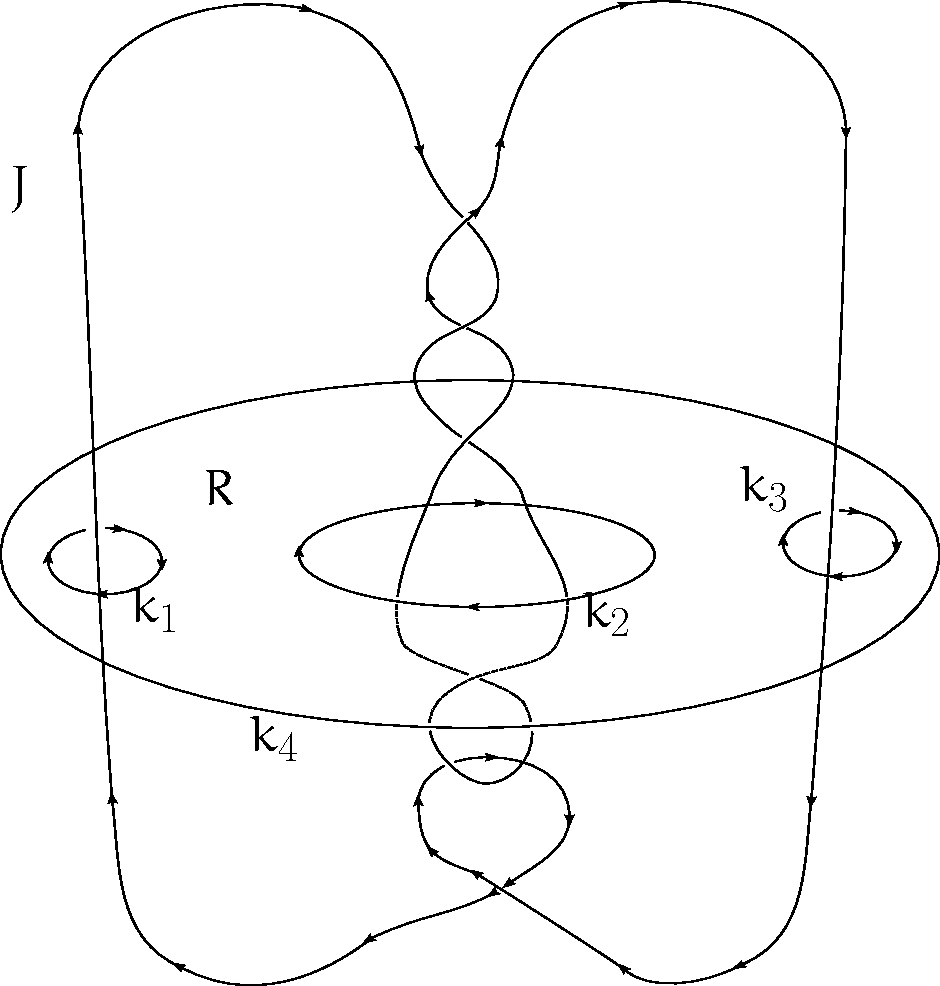
\includegraphics[width=.4\linewidth]{./pics/chap11-1-o.pdf} 
  \caption{Figure 1}
  \label{fig:11-1}
\end{figure}

If $\R{lk}(J, K)\neq 0$ then (ii) and (iii) of Proposition \ref{prop:11-13} imply that $J$ 
and $K$ cannot be deformed to manifolds separated by a hyperplane.

We shall now specialize to the classical case of knots in $\RR^3$ where $J$ and $K$ are
disjoint oriented submanifolds of $\RR^3$ diffeomorphic to $S^1$. Let us choose smooth
regular parametrizations
\begin{align*}
  \alpha:\RR\to J, && \beta:\RR\to K
\end{align*}

with periods $a$ and $b$, respectively, corresponding to a single traversing of $J$ and
$K$, respectively, agreeing with the orientation. For $p\in S^2$, consider the set
\begin{align*}
  I(p) \{(q_1, q_2)\in J\times K\big| q_2-q_1 = \lambda p, \lambda>0\}.
\end{align*}

Let $v(q_1)$ and $w(q_2)$ denote the positively oriented unit tangent vectors to $J$ and
$K$ in $q_1$ and $q_2$, respectively.


\begin{theorem}\label{theorem:11-14}
  With the notation above we have:
  \begin{enumerate}[(i)]
    \item (Gauss)
      \begin{align*}
        \R{lk}(J, K) = \frac{1}{4\pi }\int_0^a\mkern-8mu\int_0^b \frac{\det (\alpha(u) - \beta(v), \alpha'(u), \beta'(v))}
          {\|\alpha(u) - \beta(v)\|^3}
      \end{align*}
    \item There exists a dense set of points $p\in S^2$ such that
      \begin{align*}
        \det(q_1 - q_2, v(q_1), w(q_2)) \neq 0 \text{ for } (q_1, q_2)\in I(p).
      \end{align*}
    \item For such points $p$, $\R{lk}(J, K) = \sum_{(q_1, q_2)\in I(p)}^{}{\delta(q_1, q_2)}$, 
      where $\delta(q_1, q_2)$ is the sign of the determinant in (ii).
  \end{enumerate}
\end{theorem}

\begin{proof}
  We apply formula \eqref{eq:11-2} to the map $\Psi = \Psi_{J, k}$ and the volume form
$\omega = \R{vol}_{S^2}$ (with integral $4\pi$) to get
\begin{align}\label{eq:11-12}
  \R{lk}(J, k) = \R{deg}(\Psi) = \frac{1}{4\pi}\int_{J\times K}\Psi^*(\R{vol}_{S^2}).
\end{align}

We write $\Psi = r\circ f$ with 
\begin{align*}
  f:J\times K\to \RR^3 - \{0\};& \qquad f(q_1, q_2) = q_2 - q_1, \\
  r:\RR^3 - \{0\}\to S^2;& \qquad r(v) = \frac{x}{\|x\|}.
\end{align*}

For $x\in\RR^3-\{0\}, r^*(\R{vol}_{S^2})\in\alt^2(\RR^3)$ is given by 
\begin{align*}
  r^*(\R{vol}_{S^2})_x(v, w) = \det(x, v, w)\big/ \|x\|^3.
\end{align*}
(cf. Example \ref{example:9-18}). The tangent space $T_{(q_1, q_2)}(J\times K)$ has a basis 
$\{v(q_1), w(q_2)\}$, and
\begin{align*}
  Df_{(q_1, q_2)}(v(q_1)) = - v(q_1), \qquad Df_{(q_1, q_2)}(w(q_2)) = w(q_2).
\end{align*}

Therefore 
\begin{align}\label{eq:11-13}
  \Psi^*(\R{vol}_{S^2})_{(q_1, q_2)}(v(q_1)w(q_2)) 
  & = r^*(\R{vol}_{S^2})_{q_2-q_1}(-v(q_1), w(q_2))\\
  & = \|q_1 - q_2\|^{-3}\det(q_1 - q_2, v(q_1), w(q_2)).\notag
\end{align}

The integral of \eqref{eq:11-12} can be calculated by integrating $(\alpha\times\beta)^*\Psi^*(\R{vol}_{S^2})$ over 
the period rectangle $[0, a]\times [0, b]$. This yields Gauss's integral.

For $p\in S^2$, $I(p)$ is exactly the pre-image under $\Psi$. Thus $p$ is a regular value
of $\Psi$ if and only if the determinant in \eqref{eq:11-13} is non-zero for all $(q_1, q_2)\in I(p)$,
and the sign $\delta(q_1, q_2)$ is determined by whether $D_{(q_1, q_2)}\Psi$ preserves or reverses
orientation. Assertions (ii) and (iii) now follow from Theorems \ref{theorem:11-5} and \ref{theorem:11-9}. 
\end{proof}

\begin{remark}\label{remark:11-15}
  In Theorem \ref{theorem:11-14}.(ii), after a rotation of $\RR^3$ , the regular value $p$
can be assumed to be the north pole $(0, 0, 1)$. The projections of $J$ and $K$ on the
$x_1, x_2$-plane may be drawn indicating over- and undercrossings and orientations, e.g.

\begin{figure}[!htb]
  \centering
  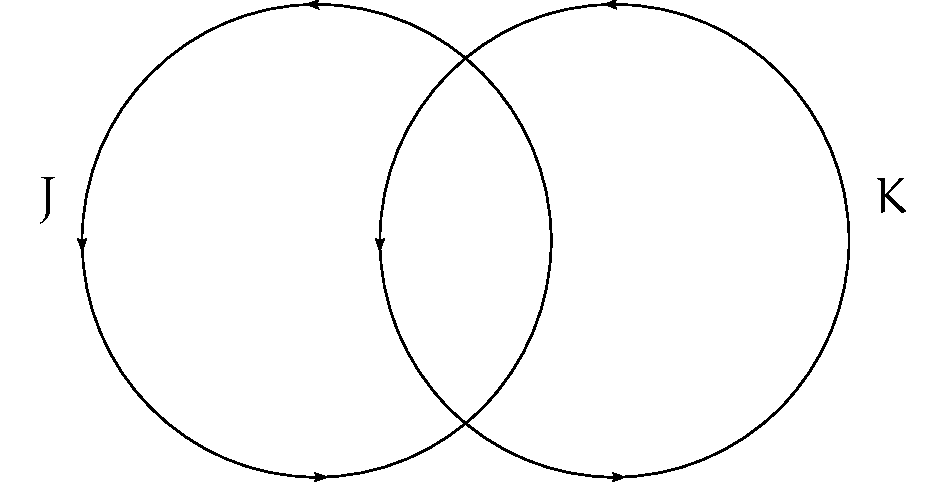
\includegraphics[width=.6\linewidth]{./pics/chap11-2-o.pdf}
  \caption{Figure 2}
  \label{fig:11-2}
\end{figure}

There is one element in $I(p)$ for every place where $K$ crosses over (and not under)
$J$. The corresponding sign $\delta$ is determined by the orientation of the curves and
of the standard orientation of the plane as shown in the picture

\begin{figure}[!htb]
  \centering
  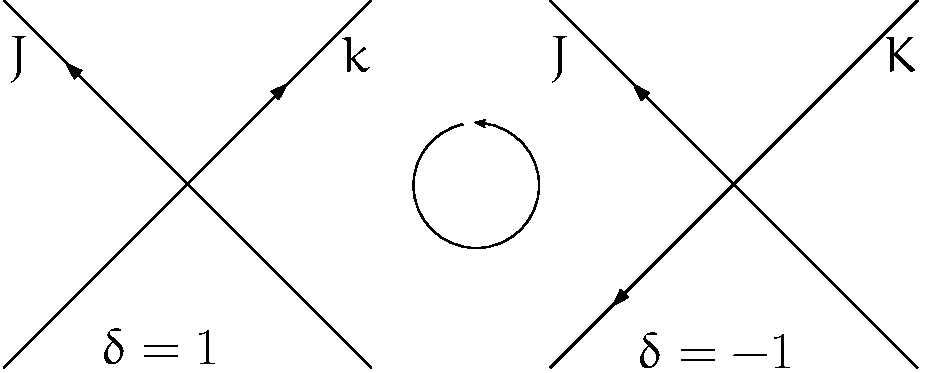
\includegraphics[width=.6\linewidth]{./pics/chap11-3-o.pdf}
  \caption{Figure 3}
  \label{fig:11-3}
\end{figure}

In Fig. \ref{fig:11-2} $\R{lk}(J, K) = -1$. In Fig. \ref{fig:11-1},
\begin{align}
  \R{lk}(J, K_2) = \R{lk}(J, k_4), \qquad \R{lk}(J, K_3) = 1,\qquad \R{lk}(J, K_1) = -1.
\end{align}
\end{remark}

We now apply the concept of degree to study singularities of vector fields.
Consider a vector field $F\in C^\infty(U, \RR^n)$ on the open set $U\sseq\RR^n, n\ge 2$, 
and let us assume that $0\in U$ is an isolated zero for $F$. A zero for $F$ is also called a
\Index{singularity} for the vector field. We can choose a $p > 0$ with
\begin{align*}
  \rho D^n = \{x\in\RR^n\big| \|x\|<\rho\}\sseq U
\end{align*}

and such that 0 is the only zero for $F$ in $\rho D^n$. Define a smooth map $F_\rho:S^{n-1}\to S^{n-1}$ 
by 
\begin{align*}
  F_\rho(x) = \frac{F(\rho x)}{\|F(\rho x)\|}.
\end{align*}

The homotopy class of $F_\rho$ is independent of the choice of $\rho$, and by Corollary
\ref{corollary:11-2} and Theorem \ref{theorem:11-9}, $\R{deg}F_\rho\in\ZZ$ is independent of $\rho$.

\begin{definition}\label{def:11-16}\index{degree}\index{local index}
  The degree of $F_\rho$ is called local index of $F$ at 0, and is denoted $\imath(F; 0)$.
\end{definition}

\begin{lemma}\label{lemma:11-17}
  Suppose $F\in C^\infty(\RR^n, \RR^n)$ has the origin as its only zero. Then 
  \begin{align*}
    F:\RR^n - \{0\}\to \RR^n - \{0\}
  \end{align*}
  induces multiplication by $\imath(F; 0)$ on $H^{n-1}(\RR^n - \{0\})\simee \RR$.
\end{lemma}

\begin{proof}
  Let $i:S^{n-1}\to\RR^n-\{0\}$ be thw inclusion map and $r:\RR^{n-1}-\{0\}\to S^{n-1}$ the 
  restriction $r(x) = x/\|x\|$. We have $\imath(F; 0) = \R{deg}F_1$, where $F_1 = r\circ F\circ i$.
  The lemma follows from the commutative diagram below, where $H^{n-1}(i)$ and $H^{n-1}(r)$ are inverse 
  isomorphisms:
  \begin{center}
    \begin{tikzcd}
      H^{n-1}(\RR^n-\{0\})\arrow[d, "H^{n-1}(r)"]\rar{H^{n-1}(F)} & H^{n-1}(\RR^n-\{0\})\arrow[d, shift left=.75ex, "H^{n-1}(i)"]\\
      H^{n-1}(S^{n-1})\rar{H^{n-1}(F_1)} & H^{n-1}(S^{n-1})\arrow[u, "H^{n-1}(r)"]
    \end{tikzcd}
  \end{center}
\end{proof}

Given a diffeomorphism $\phi:U\to V$ to an open set $V\sseq \RR^n$ and a vector field on 
$U$, we can define the direct imgae $\phi_*F \in C^\infty(V, \RR^n)$ by 
\begin{align*}
  \phi_*F(q) = D_q\phi(F(q)), p = \phi^{-1}(q).
\end{align*}

\begin{lemma}\label{lemma:11-18}
  If $F\in C^\infty(U, \RR^n)$ has 0 as an isolated singularity and $\phi:U\to V$
  is a diffeomorphism to an open set $V\sseq \RR^n$ with $\phi(0) = 0$, then 
  \begin{align*}
    \imath(\phi_*F; 0) = \imath(F, 0).
  \end{align*}
\end{lemma}

\begin{proof}
  By shrinking $U$ and $V$ we can restrict ourselves to considering the case
where 0 is the only zero for $F$ in $U$, and where there exists a diffeomorphism
$\psi:V\to\RR^n$. The assertion about $\phi$ will follow from the corresponding assertions
about $\psi$ and $\psi\circ\phi$, since
\begin{align*}
  \psi_*(\phi_*F) = (\psi\circ\phi)_*F.
\end{align*}

Thus it suffices to treat the case where $\phi:U\to \RR^n$ is a diffeomorphism and where
$Y=\phi_* F\in C^\infty(\RR^n, \RR^n)$ has the origin as its only singularity.
Let $U_0\sseq U$ be open and star-shaped around 0. We define a homotopy
\begin{align*}
  \Phi:U_0\times [0, 1]\to \RR^n; \qquad \Phi_t(x) 
    = \Phi(x, t) = \left\{\begin{aligned}
      & (D_0\phi)x && \text{ if } t = 0 \\
      & \phi(tx)/t && \text{ if } t\neq 0.
    \end{aligned}\right.
\end{align*}

For $x\in U_0$, 
\begin{align*}
  \phi(x) = \int_0^1 \frac{\dd }{\dd t}\phi(tx)\dd t 
    = \int_0^1 \left( \sum_{i=1}^{n }{x_i\frac{\partial \phi_i }{\partial x_i }(tx)} \right)\dd t
    = \sum_{i=1 }^{n }{x_i\phi_i(x)}.
\end{align*}

where $\phi_i\in C^\infty(U_0, \RR^n)$ is given by 
\begin{align*}
  \phi_i(x) = \int_0^1 \frac{\partial \phi }{\partial x_i }(tx)\dd t.
\end{align*}

It follows that
\begin{align*}
  \Phi(x, t) = \sum_{i=1 }^{n }{x_i\phi_i (tx)}
\end{align*}

and in particular that $\Phi$ has a smooth extension to an open set $W$ with
$U_0\times[0,1]\sseq W\sseq U_0\times\RR$. 

For each $t\in [0,1], \Phi_t$ is a diffeomorphism from $U_0$ to an open subset of $\RR^n$.
Consider the direct image under $\Phi_t^{-1}$ of $Y$ restricted to $\Phi_t(U_0)$:
\begin{align*}
  X_t = (\Phi_t^{-1})_*Y\in C^\infty(U_0, \RR^n) && 
  X_t(x) = (D_x\Phi_t)^{-1}Y(\Phi_t(x)).
\end{align*}

The function $X_t(x)$ is smooth on $W$. Now $X_1 = F_{|U_0}$ and $X_0 = (A^{-1})_*Y$,
where $A = D_0\phi$.

Choose $\rho>0$ such that $\rho D^n \sseq U_0$. The homotopy $S^{n-1}\times[0, 1]\to S^{n-1}$
given by 
\begin{align*}
  X_t(\rho x)\big/ \|X_t(\rho x)\|, \qquad 0\le t\le 1,
\end{align*}
and Corollary \ref{corollary:11-2} shows that 
\begin{align*}
  \imath(F; 0)
  = \imath(X_1; 0)
  = \imath(X_0; 0)
  = \imath((A^{-1})_*Y; 0).
\end{align*}

Since $A:\RR^n\to\RR^n$ is linear we have $(A^{-1})_*Y = A^{-1}\circ Y\circ A:\RR^n\to\RR^n$. This 
yields the commutative diagram 
\begin{center}
  \begin{tikzcd}
    \RR^n-\{0\}\arrow[d, "A"]\arrow[rr, "(A^{-1})_*Y"] && \RR^n-\{0\}\arrow[d, "A"]\\
    \RR^n-\{0\}\arrow[rr, "Y"] && \RR^n-\{0\}
  \end{tikzcd}
\end{center}
Now use the function $H^{n-1}$ and apply Lemma \ref{lemma:11-17} to both $Y$ and $(A^{-1})_*Y$ to 
get $\imath((A^{-1})_*Y; 0) = \imath(Y; 0)$. Hence $\imath(F; 0) = \imath(Y; 0)$.
\end{proof}

\begin{definition}\label{def:11-19}\index{local index}
  Let $X$ be a smooth tangent vector field on the manifold $M^n, n\ge 2$ with $p_0\in M$ as 
  an isolated zero. The local index $\imath(X; p_0)\in\ZZ$ of $X$ is defined by
  \begin{align*}
    \imath(X; p_0) = \imath(h_*X_{|U}; 0),
  \end{align*}
  where $(U, h)$ is an arbitrary chart around $p_0$ with $h(p_0) = 0$.
\end{definition}

We note that Lemma \ref{lemma:11-18} shows that the local index does not depend on the
choice of $(U, h)$. One can picture vector fields in the plane by drawing their
integral curves, e.g.

\begin{figure}[!htb]
  \centering
  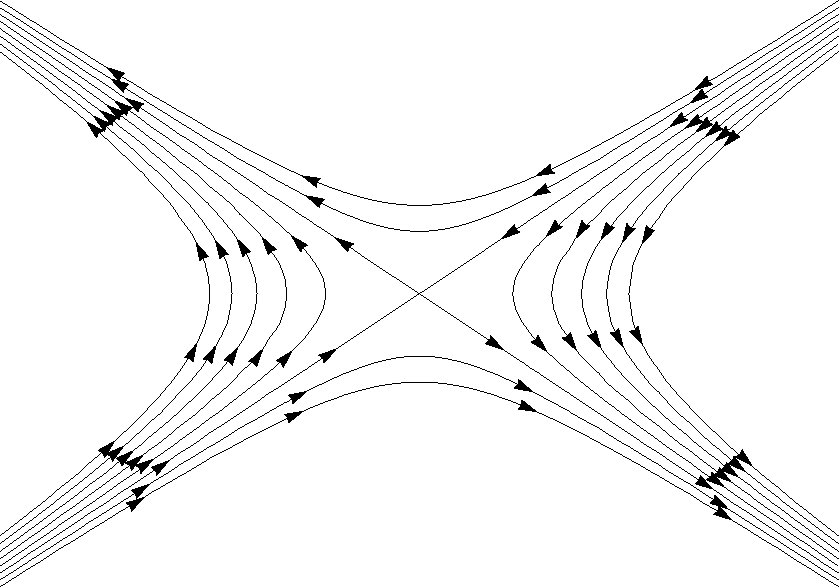
\includegraphics[width=.4\linewidth]{./pics/chap11-4-I.pdf}\quad
  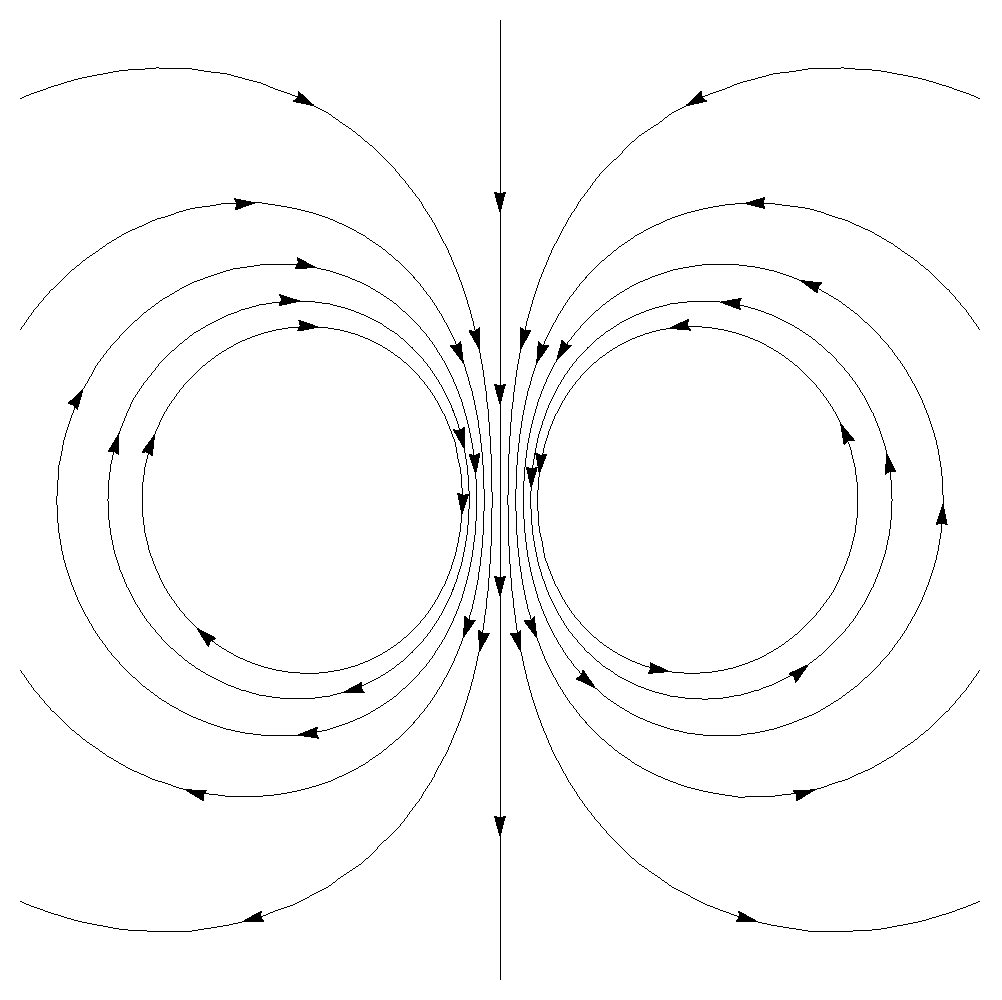
\includegraphics[width=.4\linewidth]{./pics/chap11-4-II.pdf}
  \caption{Figure 4}
  \label{fig:11-4}
\end{figure}

Let $X$ be a smooth tangent vector field on Mn and let $p_0\in M^n$ be a zero. Let
\begin{align*}
  F = h_*(X_{|U})\in C^\infty(\RR^n, \RR^n)
\end{align*}

for a chart $(U, h)$ with $h(p_0) = 0$. If $D_0F:\RR^n\to\RR^n$ is an isomorphism, then
$p_0$ is said to be a non-degenerate singularity or zero\index{non-degenarate zero}. Note that by the inverse
function theorem $F$ is a local diffeomorphism around 0, such that 0 is an isolated
zero for $F$. Hence $p_0\in M^n$ is also an isolated zero for $X$.

\begin{lemma}\label{lemma:11-20}
  If $p_0$ is a non-degenerate singularity, then
  \begin{align*}
    \imath(X, p_0) = \R{sign}(\det D_0F)\in \{\pm 1\}.
  \end{align*}
\end{lemma}

\begin{proof}
  By shrinking $U$ we may assume that $h$ maps $U$ diffeomorphically onto an
open set $U_0\in\RR^n$, which is star-shaped around 0, and that $F$ is a diffeomorphism
from $U_0$ to an open set. As in the proof of Lemma \ref{lemma:11-18} we can define a homotopy
\begin{align*}
  G:U_0\times[0, 1]\to\RR^n; \qquad G(x, t) = \left\{\begin{aligned}
    & D_0F   && \text{ if } t = 0 \\
    & F(tx)/t && \text{ if } t\neq 0.
  \end{aligned}\right.
\end{align*}

where $G$ can be extended smoothly to an open set $W$ in $U_0\times \RR$ that contains
$U_0\times [0,1]$. Choose $p > 0$ so that $\rho D^n\sseq U_0$. We get a homotopy $\tilde{G}:
S^{n-1}\times[0, 1]\to S^{n-1}$,
\begin{align*}
  \tilde{G}(x, t) = G(\rho x, t)\big/ \|G(\rho x, t)\|.
\end{align*}

between the map $F_\rho$ in Definition \ref{def:11-16} and the analogous map $A_\rho$ with $A=D_0F$.
It follows from Corollary \ref{corollary:11-2} that
\begin{align*}
  \imath(X; p_0) = \imath(F; 0) 
  = \R{deg}(F_\rho) = \R{deg}A_\rho  
  = \imath(A; 0).
\end{align*}

The map $f_A:\RR^n-\{0\}\to \RR^n-\{0\}$ induced by $A$ operates on $H^{n-1}(\RR^n-\{0\})$ by 
multiplication by $\imath(X; p_0)$; cf. Lemma \ref{lemma:11-17}. The result follows from 
Lemma \ref{lemma:6-14}.
\end{proof}

\begin{definition}\label{def:11-21}
  Let $X$ be a smooth vector field on $M^n$, with only isolated
  singularities. For a compact set $R\sseq M$ we define the total index of $X$ over
  $R$ to be
  \begin{align*}
    \R{Index}(X; R) = \sum \imath(X; p)
  \end{align*}
  where the summation runs over the finite number of zeros $p\in R$ for $X$. If $M$ is
  compact we write Index $(X)$ instead of Index $(X; M)$.
\end{definition}

\begin{theorem}\label{theorem:11-22}
  Let $F\in C^\infty(U, \RR)$ be a vector field on an open set $U\sseq\RR^n$,
with only isolated zeros. Let $R\sseq U$ be a compact domain with smooth boundary
$\partial R$, and assume that $F(p)\neq 0$ for $p\in\partial R$. Then
\begin{align*}
  \R{Index}(F; R) = \R{deg}(f),
\end{align*}
where $f:\partial R\to S^{n-1}$ is the map $f(x) = F(x)/\|F(x)\|$.
\end{theorem}

\begin{proof}
  Let $p_1, \cdots, p_k$ be the zeros in $R$ for $F$, and choose disjoint closed balls
$D_j\sseq R-\partial R$, with centers $p_j$. Define
\begin{align*}
  f_j: \partial D_j \to S^{n-1}; \qquad f_j(x) = F(x)/\|F(x)\|.
\end{align*}

We apply Proposition \ref{prop:11-11} with $X = R-\cup_{j}\mrg{D}_j$. The boundary $\partial x$ 
is the disjoint union of aR and the $(n - 1)$-spheres $\partial D_1, \cdots, \partial D_k$. Here $\partial D_j$, 
considered as boundary component of $X$, has the opposite orientation to the one induced from $D_j$. 
Thus
\begin{align*}
  \R{deg}(f) + \sum_{j=1}^{k}{-\R{deg}(f_j)} = 0.
\end{align*}

Finally $\R{deg}(f_j) = \imath(F; p_j)$ by the definition of local index and Corollary \ref{corollary:11-3}.
\end{proof}

\begin{corollary}\label{corollary:11-23}
  In the situation of Theorem \ref{theorem:11-22}, $\R{Index}(F; R)$ depends only on
the restriction of $F$ to $\partial R$.
\end{corollary}

\begin{corollary}\label{corollary:11-24}
  In the situation of Theorem \ref{theorem:11-22}, suppose for every $p\in\partial R$ that
  the vector $F(p)$ points outward. Let $g:\partial R\to S^{n-1}$ be the Gauss map which to
  $p\in\partial R$ associates the outward pointing unit normal vector to $\partial R$. Then
  \begin{align*}
    \R{Index}(F; R) = \R{deg}(g).
  \end{align*}
\end{corollary}

\begin{proof}
  By Corollary \ref{corollary:11-2} it sufficies to show that $f$ and $g$ are homotopic. Since
  $f(p)$ and $g(p)$ belong to the same open half-space of $\RR^n$ , the desired homotopy
  can be defined by
  \begin{align*}
    \frac{(1-t)f(p) + tg(p)}{\|(1-t)f(p) + tg(p)\|}.\qquad (0\le t\le 1).
    \tag*{\qedsymbol}
  \end{align*}
\end{proof}

\begin{lemma}\label{lemma:11-25}
  Suppose $F\in C^\infty(\RR^n, \RR^N)$ has the origin as its only zero. Then
  there exists an $F\in C^\infty(\RR^n, \RR^N)$, with only non-degenerate zeros, that coincides
  with $F$ outside a compact set.
\end{lemma}

\begin{proof}
  We choose a function $\phi\in C^\infty(\RR^n, [0, 1])$ with 
  \begin{align*}
    \phi(x) = \left\{\begin{aligned}
      & 1 && \text{ if } \|x\|\le 1 \\
      & 0 && \text{ if } \|x\|\ge 2.
    \end{aligned}\right.
  \end{align*}
  We want to define $\tilde{F}(x) = F(x) - \phi(x)w$ for a suitable $w\in\RR^n$. 
  For $\|x\|> 2$ we have $\tilde{F}(x) = F(x)$. Set
  \begin{align*}
    c = \inf_{1\le \|x\|\le 2} \|F(x)\| > 0
  \end{align*}
  and choose $w<c$. For $1\le\|x\|\le 2, \|\tilde{F}(x)\|\ge c-\|w\|>0$. Thus all 
  zeros of $\tilde{F}$ belong to the open unit ball $D^n$. Since $\tilde{F}$ coincides with 
  $F-w$ on $\mrg{D}^n$ 
  \begin{align*}
    \tilde{F}^{-1}(0) = \mrg{D}^n\cap F^{-1}(w).
  \end{align*}
  We can pick $w$ as a regular value of $F$ with $\|w\|<c$ by Sard's theorem. Then
  $D_p\tilde{F} = D_pF$ will be invertible for all $p\in\tilde{F}^{-1}(0)$, and $P$ has 
  the desired properties.
\end{proof}

Note, by Corollary \ref{corollary:11-23}, that
\begin{align}
  \imath(F; 0) = \sum_{p\in \tilde{F}^{-1}(p)}^{}{\imath(\tilde{F}, p)}
\end{align}

Here is a picture of $F$ and $\tilde{F}$ in a simple case:
\begin{figure}[!htb]
  \centering
  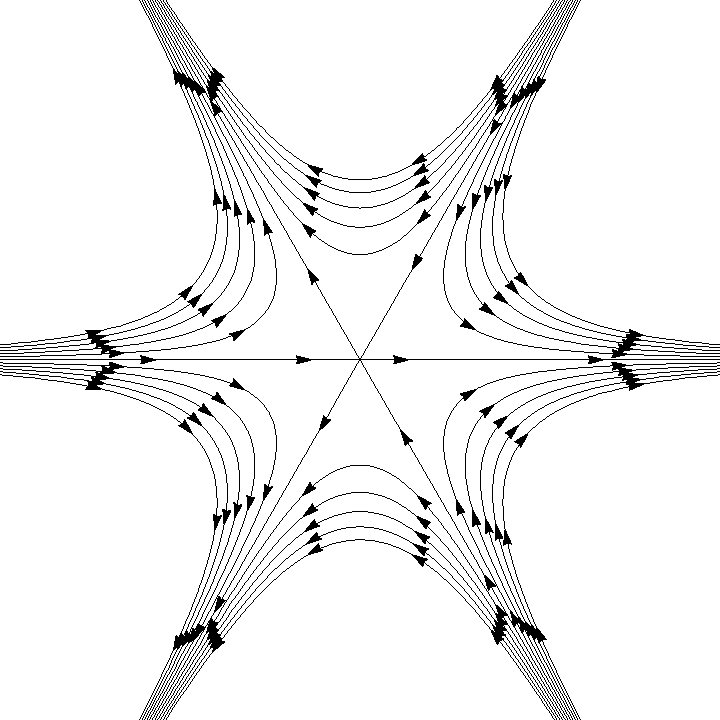
\includegraphics[width=.4\linewidth]{./pics/chap11-5-I.pdf}\quad
  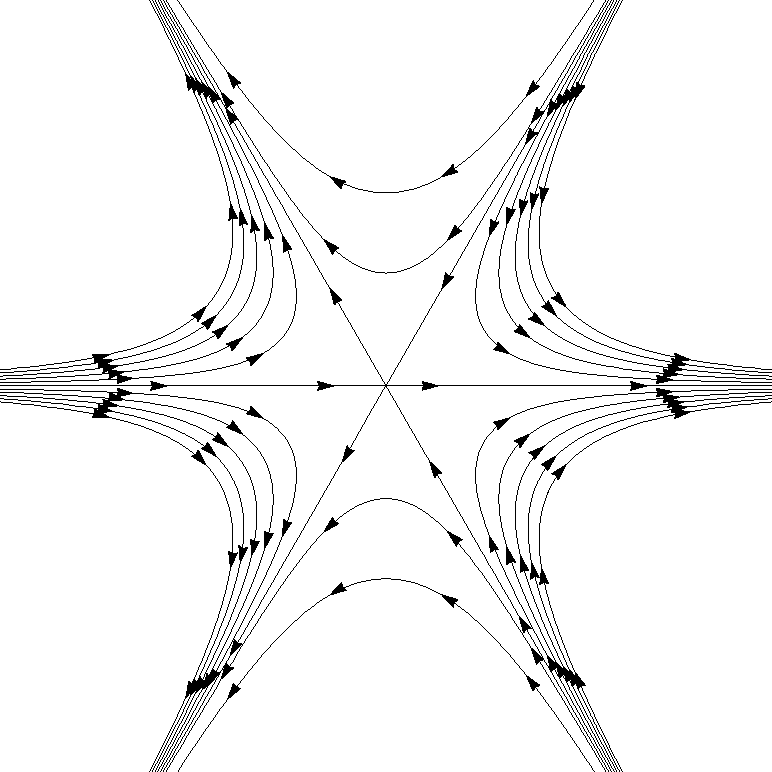
\includegraphics[width=.4\linewidth]{./pics/chap11-5-II.pdf}
  \caption{Figure 5(Left--$F$; Right--$\tilde{F}$)}
  \label{fig:11-5}
\end{figure}

The zero for $F$ of index -2 has been replaced by two non-degenerate zeros for
$\tilde{F}$, both of index -1.

\begin{corollary}\label{corollary:11-26}
  Let $X$ be a smooth vector field on the compact manifold $M^n$
with isolated singularities. Then there exists a smooth vector field $\tilde{X}$ on $M$ having
only non-degenerate zeros and with
\begin{align}\label{eq:11-14}
  \R{Index}(X) = \R{Index}(\tilde{X}).
\end{align}
\end{corollary}

\begin{proof}
  We choose disjoint coordinate patches which are diffeomorphic to $\RR^n$
around the finitely many zeros of $X$, and apply Lemma \ref{lemma:11-25} on the interior of
each of them to obtain $\tilde{X}$. The formula then follows from \eqref{eq:11-14}.
\end{proof}

\begin{theorem}\label{theorem:11-27}
  Let $M^n\sseq\RR^n$ be a compact smooth submanifold and let $N_\epsilon$ be
a tubular neighborhood of radius $\epsilon>0$ around $M$. Denote by $g:\partial N_\epsilon\to S^{n+k-1}$
the outward pointing Gauss map. If $X$ is an arbitrary smooth vector field on $M^n$
with isolated singularities, then
\begin{align*}
  \R{Index}(X) = \R{deg}(g).
\end{align*}
\end{theorem}

\begin{proof}
  By Corollary \ref{corollary:11-26} one may assume that $X$ only has non-degenerate zeros.
From the construction of the tubular neighborhood we have a smooth projection
$\pi: N\to M$ from an open tubular neighborhood $N$ with $N_\epsilon\sseq N\sseq \RR^{n+k}$, and 
can define a smooth vector field $F$ on $N$ by
\begin{align}\label{eq:11-15}
  F(q) = X(\pi(q)) + (q - \pi(q)).
\end{align}

ince the two summands are orthogonal, $F(q) = 0$ if and only if $q\in M$ and
$X(q) = 0$. For $q\in\partial N_\epsilon, q-\pi(q)$ is a vector normal to $T_q\partial N_\epsilon$ 
pointing outwards. Hence $X(\pi(q))\in T_q\partial N_\epsilon$ and $F(q)$ points outwards. 
By Corollary \ref{corollary:11-24} 
\begin{align*}
  \R{Index}(F; N) = \R{deg}(g).
\end{align*}

and it suffices to show that $\imath(X; p) = \imath(F; p)$ for an arbitrary zero of $X$. In 
local coordinates around $p$ in $M$, with $p$ corresponding to $0\in\RR^n$, $X$ can be written
in the form
\begin{align}\label{eq:11-16}
  X = \sum_{i=1}^{n}{f_i(x) \frac{\partial }{\partial x_i }},
\end{align}

where $f_i(0) = 0$, and by Lemma \ref{lemma:11-20} $\imath(X; p)$ is the sign of 
\begin{align}\label{eq:11-17}
  \det\left(\frac{\partial f_i }{\partial x_j }(0)\right).
\end{align}

By differentiating \eqref{eq:11-16} and substituting 0 one gets
\begin{align}\label{eq:11-18}
  \frac{\partial X }{\partial x_j }(0) 
  = \sum_{i=1 }^{n }{\frac{\partial f_i }{\partial x_j }(0) \frac{\partial }{\partial x_i }}.
\end{align}

It follows from \eqref{eq:11-15} that $D_pF:\RR^{n+k}\to\RR^{n+k}$ is the identity 
on $T_pM^\perp$ and by \eqref{eq:11-18} $D_pF$ maps $T_pM$ into itself by the linear map with 
matrix ($(\partial f_i/\partial x_i)(0)$) (with respect to the basis $(\partial/\partial x_i)_0$). 
It follows that $p$ is a non-degenerate zero for $F$ and that $\det D_pF$ has the same sign as 
the Jacobian in \eqref{eq:11-17}.
\end{proof}